\documentclass[10pt, uplatex, dvipdfmx]{jsarticle}
\usepackage{../mypackage}

\graphicspath{{../pictures}}

\setcounter{section}{8}

\begin{document}

\section{2重積分の計算(変数変換)}


偏微分可能な $2$ 変数関数 $\varphi,\psi$ による変数変換 $
\begin{cases}
  x=\varphi(u,v)\\
  y=\psi(u,v)
\end{cases}
$ に対して,$u,v$ に関する $2$ 変数関数
\[
  J(u,v) = \left|
    \begin{array}{cc}
      \frac{\partial x}{\partial u} & \frac{\partial x}{\partial v}\\[1ex]
      \frac{\partial y}{\partial u} & \frac{\partial y}{\partial v}
    \end{array}
  \right|=\frac{\partial x}{\partial u} \frac{\partial y}{\partial v}
  - \frac{\partial x}{\partial v} \frac{\partial y}{\partial u}
  \; \Big( = \varphi_{u} \psi_{v} - \varphi_{v}\psi_{u}\Big)
\]
をこの変換の Jacobian という.Jacobian は以下のように書かれることもあ
る.
\[
  \frac{D(x,y)}{D(u,v)}, \quad \frac{\partial(x,y)}{\partial(u,v)}
\]

\subsection{変数変換の公式}

\begin{theorem}\label{thm:iint-trans}
  $uv$ 平面の閉領域 $E$ から $xy$ 平面の閉領域 $D$ への1対1の変数変換
  (全単射)
  \[
    \Phi:
    \begin{cases}
      x=\varphi(u,v)\\
      y=\psi(u,v)
    \end{cases}
    \quad \left(\text{ $\varphi, \psi$ は $C^1$ 級} \right)
  \]
  の Jacobian を $J(u,v)$ とし,全ての $(u,v) \in E$ に対して $J(u,v)
  \neq 0$ とする.このとき $D$ 上積分可能な連続関数 $f(x,y)$ に対して以下が成り
  立つ.
  \begin{equation}\label{eq:iint-trans}
    \iint_{D} f(x,y) \ dx dy 
    = \iint_{E} f\left( \varphi(u,v), \psi(u,v)\right) \left| J(u,v)\right| du dv
  \end{equation}
  \begin{figure}[b]
    \centering
    \includegraphics[height=8.5cm]{09/uv2xy.pdf}
  \end{figure}
\end{theorem}




\begin{example}
  次の重積分の計算に定理\ref{thm:iint-trans}を適用してみよう.
  \[
    \iint_{D} x^2 \ dx dy,  \quad D=\Set{(x,y) | \ |x+2y| \leqq 1, \, |x-y| \leqq 1}
  \] 

  $u=x+2y, \, v=x-y$ とおく.すなわち,変数変換
  \[
    \Phi :
    \begin{cases}
      x=\frac{1}{3}u+\frac{2}{3}v\\[1ex]
      y=\frac{1}{3}u-\frac{1}{3}v
    \end{cases}
  \]
  を考える.$\Phi$ は下図のように $uv$ 平面の閉領域
  \[
    E=\Set{(u,v) | -1 \leqq u \leqq 1, \, -1 \leqq v \leqq 1}
  \]
  から $xy$ 平面の閉領域 $D$ への1対1の写像である.
  \begin{figure}[h]
    \centering
    \begin{tabular}[h]{ccc}
      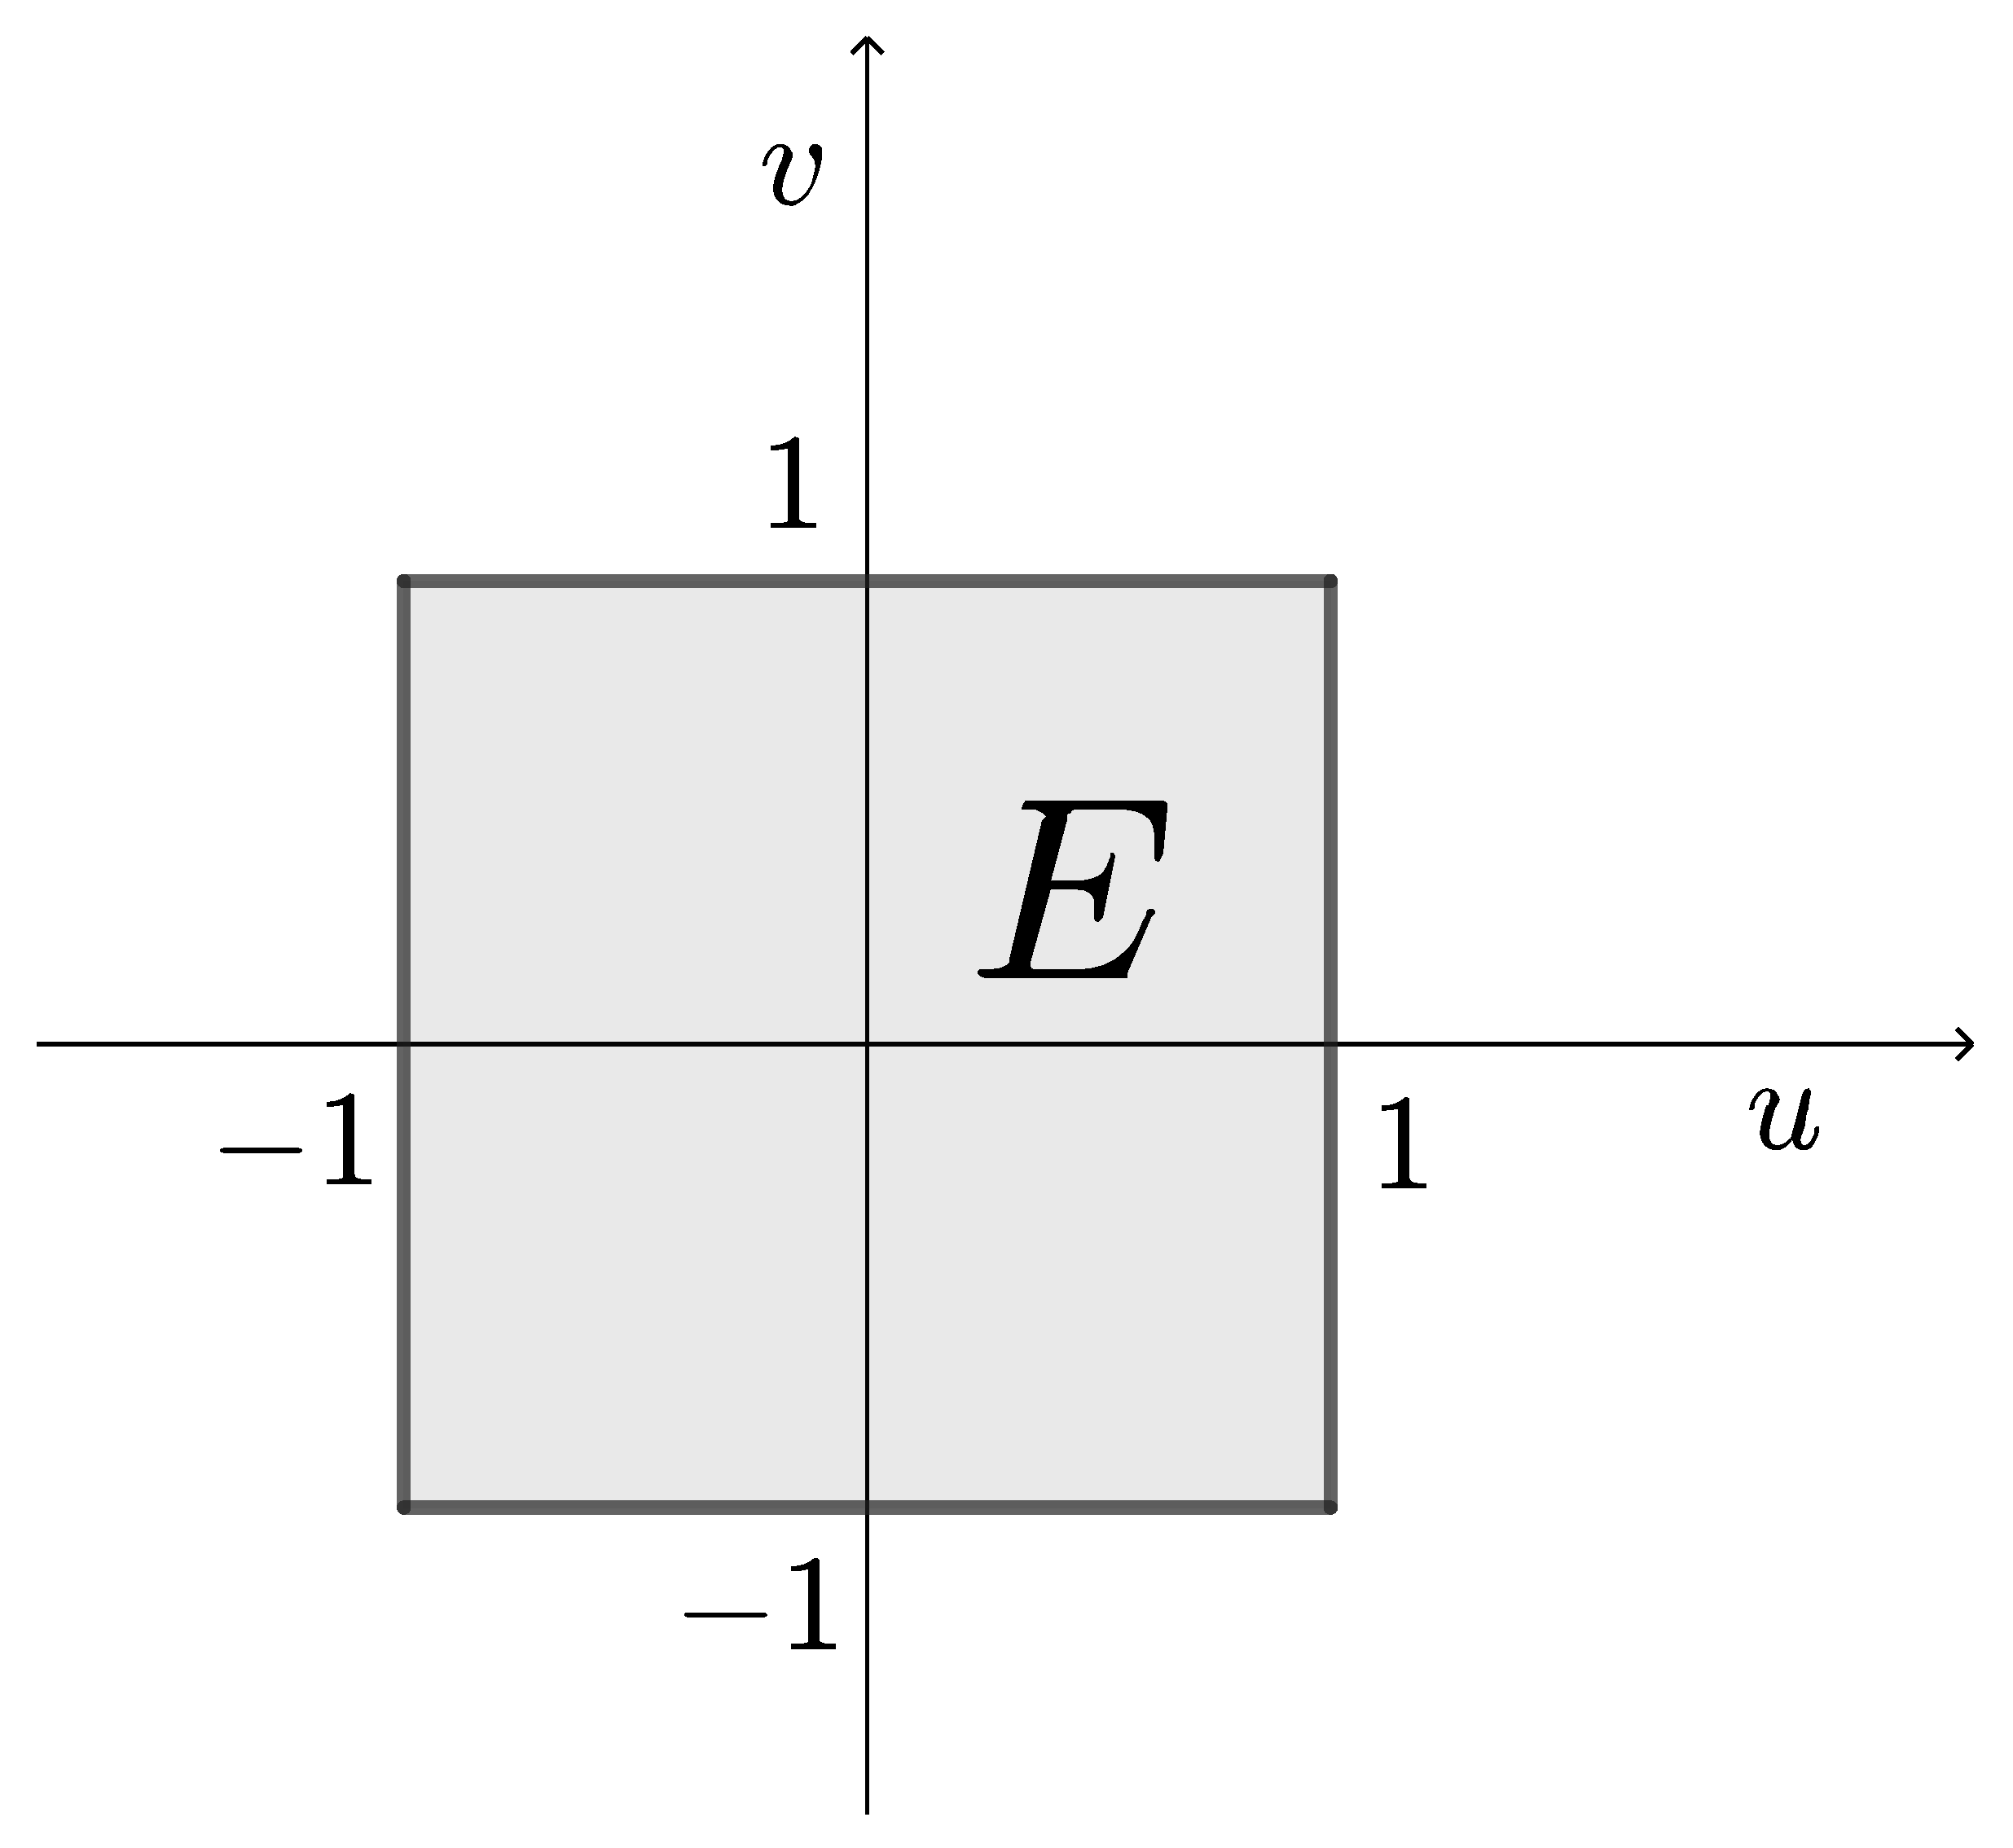
\includegraphics[height=5cm]{09/ex1uv.pdf}
      & \multirow{1}{*}[2.1cm]{$\overset{\Phi}{\longrightarrow}$}
      &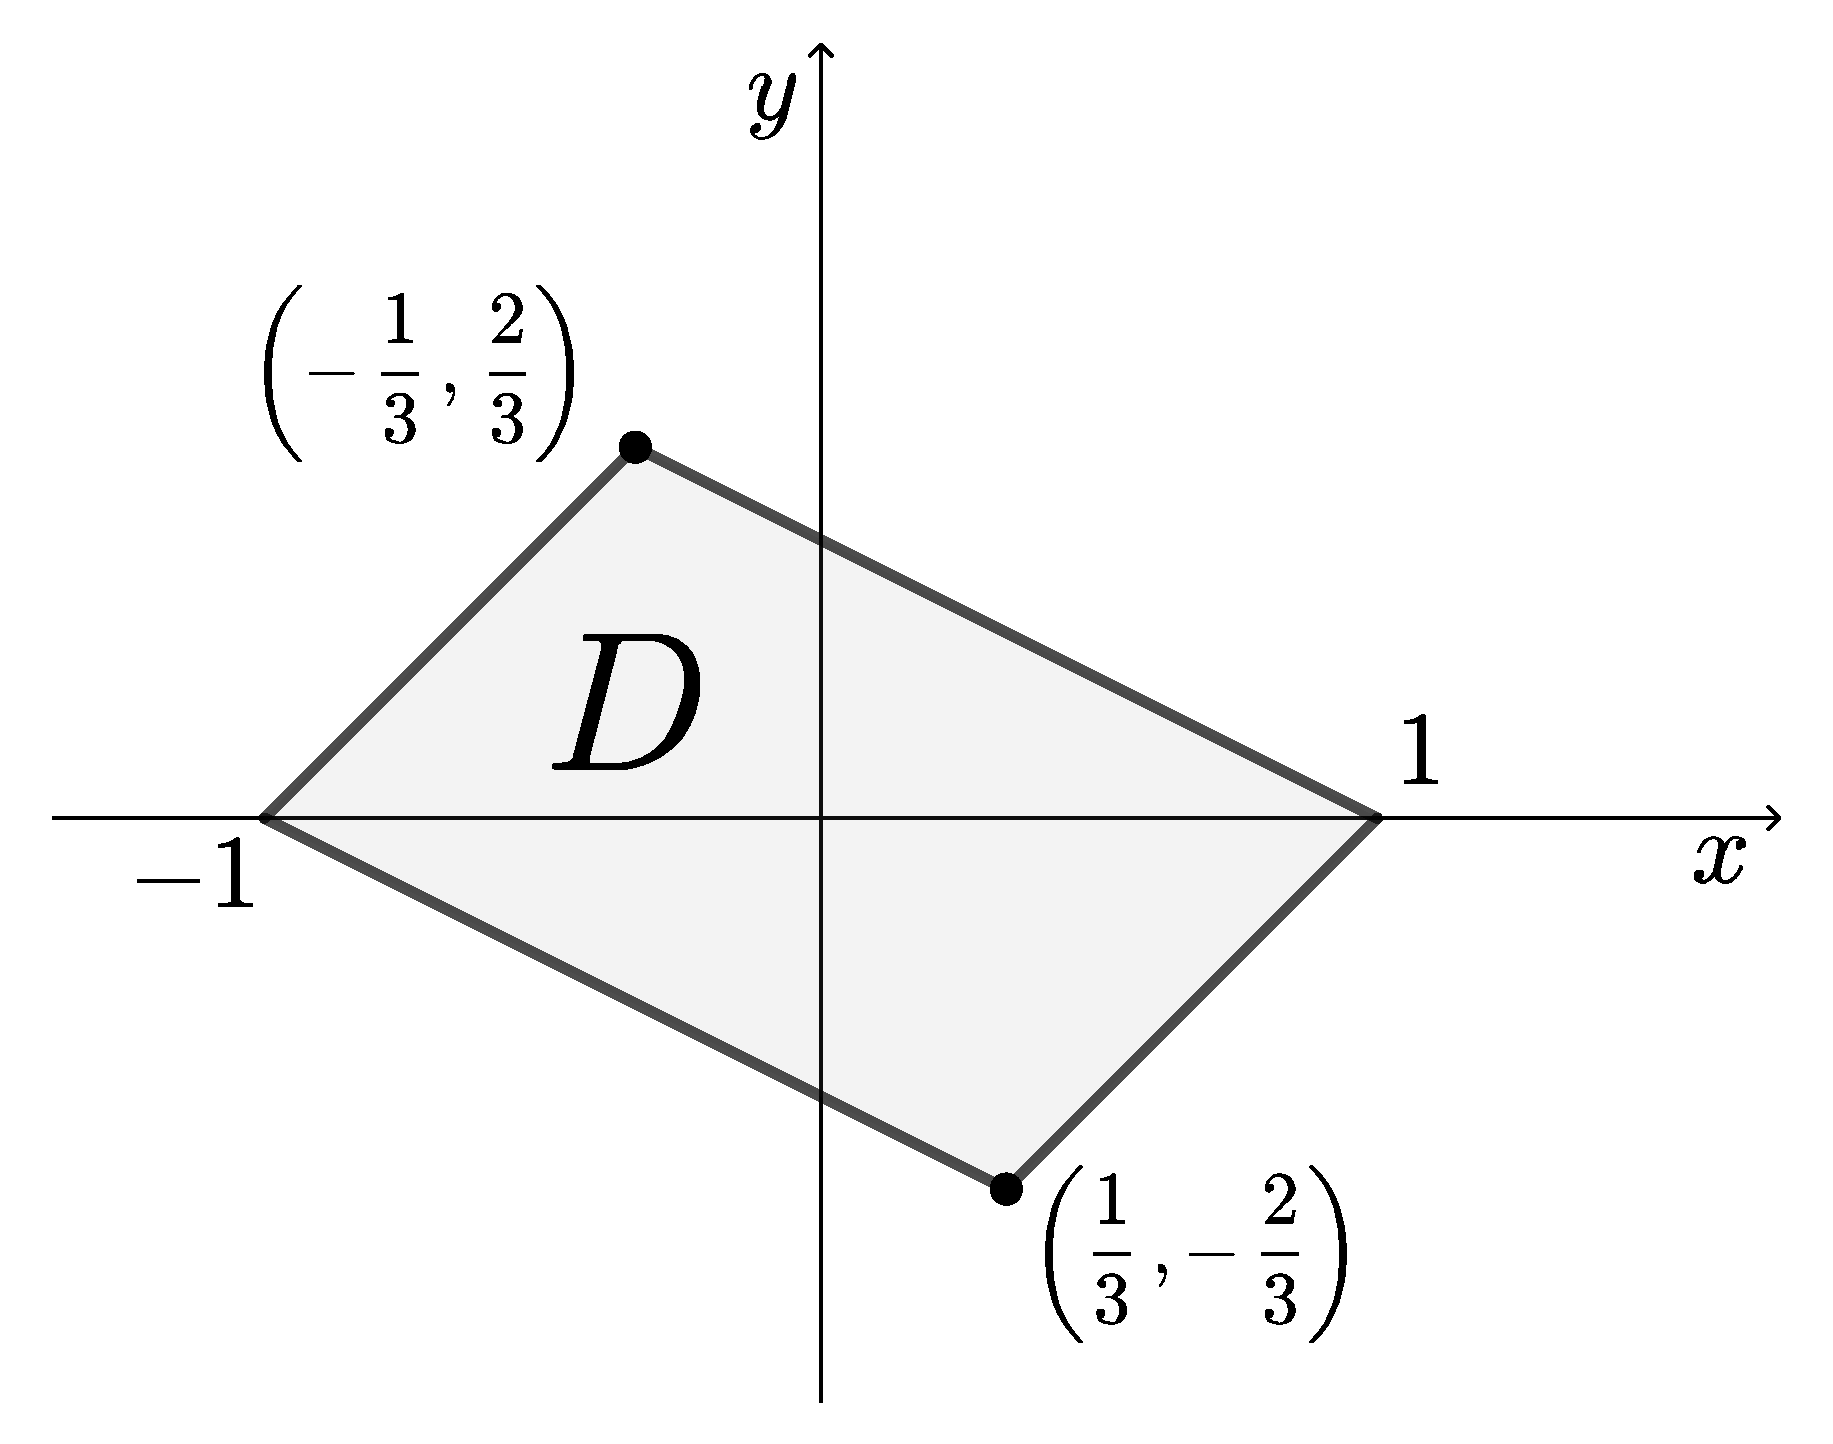
\includegraphics[height=5cm]{09/ex1xy.pdf}
    \end{tabular}
  \end{figure}

  \noindent
  変数変換 $\Phi$ の Jacobian は
  \[
    J(u,v) = \left|
      \begin{array}{cc}
        \frac{\partial x}{\partial u} & \frac{\partial x}{\partial v}\\[1ex]
        \frac{\partial y}{\partial u} & \frac{\partial y}{\partial v}
      \end{array}
    \right| =\left|
      \begin{array}{rr}
        \frac{1}{3} & \frac{2}{3}\\
        \frac{1}{3} & -\frac{1}{3}
      \end{array}
    \right| = -\frac{1}{3}
  \]
  であるから,$(u,v) \in E$ に対して $J(u,v) \neq 0$ である.よっ
  て,定理\ref{thm:iint-trans}より以下を得る.
  \begin{align*}
    \iint_{D} x^2 \ dx dy
    &= \iint_{E} \left( \frac{1}{3}u+\frac{2}{3}\right)^2 \left| J(u,v)\right| \ du dv
    =\iint_{E} \frac{1}{3}\left( \frac{1}{3}u+\frac{2}{3}\right)^2  du dv\\
    &= \frac{1}{27}\int_{-1}^{1} \left( \int_{-1}^{1} \left( u+2v\right)^2 du \right) dv
    =\frac{1}{27}\int_{-1}^{1} \left[ \frac{1}{3} \left( u+2v\right)^3 \right]_{u=-1}^{u=1} dv\\
    &=\frac{1}{81} \int_{-1}^{1} \left( \left( 2v+1\right)^3 -\left(2v-1\right)^3\right) dv
      = \frac{1}{81} \left[ \frac{(2v+1)^4}{8}- \frac{(2v-1)^4}{8}\right]_{-1}^{1}\\
    &=\frac{20}{81}
  \end{align*}

\end{example}

\newpage

\begin{remark}
  定理\ref{thm:iint-trans}の最後の等式 (\ref{eq:iint-trans}) は,変数変
  換 $\Phi$ が $E$ の面積 $0$ の部分集合 $N$ を除いて1対1で,$(u,v)
  \notin N$ に対して $J(u,v) \neq 0$ であれば成立する.
\end{remark}

例えば,正の実数 $R$ に対し極座標変換
\[
  \begin{cases}
    x = r \cos \theta\\
    y = r \sin \theta
  \end{cases}
\]
は下図のように $r\theta$ 平面の閉領域
\[
  E=\Set{ (r,\theta) | 0 \leqq r \leqq R, \, 0 \leqq \theta \leqq 2\pi}
\]
から $xy$ 平面の閉領域
\[
  D=\Set{(x,y) | x^2+y^2 \leqq R^2}
\]
への変換を与えるが,これは1対1の対応ではない.しかしながら,
\[
  N=\Set{(r, \theta) \in E | r=0} \cup \Set{(r,\theta) | \theta=2\pi}
\]
とおけば,$N$ は $E$ の面積 $0$ の部分集合であり,極座標変換は $E-N$
から $D-\Set{(0,0)}$ への1対1の対応(全単射)を与える.
\begin{figure}[h]
  \centering
  \includegraphics[height=6cm]{09/polar.pdf}
\end{figure}

\noindent
このとき,極座標変換
の Jacobian は
\[
  J(r, \theta) = \left|
    \begin{array}{cc}
      \frac{\partial x}{\partial r} & \frac{\partial x}{\partial \theta}\\[1ex]
      \frac{\partial y}{\partial r} & \frac{\partial y}{\partial \theta}
    \end{array}
  \right| = \left|
    \begin{array}{rr}
      \cos \theta & -r\sin\theta\\
      \sin \theta & r \cos \theta
    \end{array}
  \right| = r
\]
であるから,$(r, \theta) \notin N$ ならば $J(r, \theta) \neq 0$ であ
る.従って,$D$ 上重積分可能な $2$ 変数関数 $f(x,y)$ に対して,以下が成り立つ.
\[
  \iint_{D}f(x,y)\ dx dy = \iint_{E} f\left( r\cos\theta, r\sin\theta\right) r \ dr d\theta
\]

\newpage

\subsection{練習問題}


次の2重積分を求めよう.

\vspace{1zh}

\begin{enumerate}[(1)]

  \setlength{\itemsep}{2zh}
  
\item $\ds \iint_{D} (x^2-y^2)\ dx dy, \quad
  D=\Set{(x,y) | 1 \leqq x+y \leqq 2, \, 0 \leqq x-y \leqq 1}$

\item $\ds \iint_{D} e^{-x^2-y^2} dx dy, \quad
  D=\Set{(x,y) | 1 \leqq x^2+y^2 \leqq 9}$

\item $\ds \iint_{D} \sqrt{x^2+y^2}\ dx dy, \quad
  D=\Set{(x,y) | 0 \leqq y \leqq x^2+y^2 \leqq 1, \, 0 \leqq x}$

\item $\ds \iint_{D} (x^2+y^2)\ dx dy, \quad
  D=\Set{(x,y) | \frac{x^2}{4}+ \frac{y^2}{9} \leqq 1 }$

\item $\ds \iint_{D} xy\ dx dy, \quad D=\Set{(x,y) | \sqrt{x} + \sqrt{y} \leqq 1}$

\end{enumerate}


\vspace{3zh}

「積分基本問題集 弍」(5) $\sim$ (10), (12), (13) も参考にしてください.
\begin{center}
  \url{https://github.com/kazutsumi/Integral2/blob/main/integral2.pdf}
\end{center}


\begin{figure}[b]
  答え:(1) $\ds \frac{3}{8}$ \quad (2) $\ds \pi\left(e^{-1}-e^{-9}\right)$ \quad (3) $\ds \frac{\pi}{6}-\frac{2}{9}$ \quad
  (4) $\ds \frac{39\pi}{2}$ \quad (5) $\ds \frac{1}{280}$
\end{figure}




\end{document}
